%%%%%%%%%%%%%%%%%%%%%%%%%%%%%%%%%%%%%%%%%
% Beamer Presentation
% LaTeX Template
% Version 1.0 (10/11/12)
%
% This template has been downloaded from:
% http://www.LaTeXTemplates.com
%
% License:
% CC BY-NC-SA 3.0 (http://creativecommons.org/licenses/by-nc-sa/3.0/)
%
%%%%%%%%%%%%%%%%%%%%%%%%%%%%%%%%%%%%%%%%%

%----------------------------------------------------------------------------------------
%	PACKAGES AND THEMES
%----------------------------------------------------------------------------------------

\documentclass{beamer}

\usepackage{minted}
\usepackage{float}
\usepackage{caption}

\mode<presentation> {

% The Beamer class comes with a number of default slide themes
% which change the colors and layouts of slides. Below this is a list
% of all the themes, uncomment each in turn to see what they look like.

%\usetheme{default}
%\usetheme{AnnArbor}
%\usetheme{Antibes}
%\usetheme{Bergen}
%\usetheme{Berkeley}
%\usetheme{Berlin}
%\usetheme{Boadilla}
%\usetheme{CambridgeUS}
%\usetheme{Copenhagen}
%\usetheme{Darmstadt}
%\usetheme{Dresden}
%\usetheme{Frankfurt}
%\usetheme{Goettingen}
%\usetheme{Hannover}
%\usetheme{Ilmenau}
%\usetheme{JuanLesPins}
%\usetheme{Luebeck}
%\usetheme{Madrid}
%\usetheme{Malmoe}
%\usetheme{Marburg}
%\usetheme{Montpellier}
%\usetheme{PaloAlto}
%\usetheme{Pittsburgh}
%\usetheme{Rochester}
%\usetheme{Singapore}
%\usetheme{Szeged}
\usetheme{Warsaw}

% As well as themes, the Beamer class has a number of color themes
% for any slide theme. Uncomment each of these in turn to see how it
% changes the colors of your current slide theme.

%\usecolortheme{albatross}
%\usecolortheme{beaver}
%\usecolortheme{beetle}
%\usecolortheme{crane}
%\usecolortheme{dolphin}
%\usecolortheme{dove}
%\usecolortheme{fly}
%\usecolortheme{lily}
%\usecolortheme{orchid}
%\usecolortheme{rose}
%\usecolortheme{seagull}
%\usecolortheme{seahorse}
%\usecolortheme{whale}
%\usecolortheme{wolverine}

%\setbeamertemplate{footline} % To remove the footer line in all slides uncomment this line
\setbeamertemplate{footline}[page number] % To replace the footer line in all slides with a simple slide count uncomment this line

\setbeamertemplate{navigation symbols}{} % To remove the navigation symbols from the bottom of all slides uncomment this line
}

\usepackage{graphicx} % Allows including images
\usepackage{booktabs} % Allows the use of \toprule, \midrule and \bottomrule in tables

%----------------------------------------------------------------------------------------
%	TITLE PAGE
%----------------------------------------------------------------------------------------

\title{Razvoj SUPB z integracijo v programski jezik Python} % The short title appears at the bottom of every slide, the full title is only on the title page

\author{Janez Sedeljšak
\\ Mentor: doc. dr. Boštjan Slivnik
\\ Somentor: asist. dr. Marko Poženel
} % Your name
\institute[UL FRI] % Your institution as it will appear on the bottom of every slide, may be shorthand to save space
{
Univerza v Ljubljani, Fakulteta za računalništvo in informatiko \\ % Your institution for the title page
\medskip
\textit{js0578@student.uni-lj.si} % Your email address
}
\date{\today} % Date, can be changed to a custom date

\begin{document}

\begin{frame}
\titlepage % Print the title page as the first slide
\end{frame}

\setcounter{tocdepth}{1}

\begin{frame}
\frametitle{Kazalo} % Table of contents slide, comment this block out to remove it
\tableofcontents % Throughout your presentation, if you choose to use \section{} and \subsection{} commands, these will automatically be printed on this slide as an overview of your presentation
\end{frame}

%----------------------------------------------------------------------------------------
%	PRESENTATION SLIDES
%----------------------------------------------------------------------------------------

%------------------------------------------------
\section{Uvod} % Sections can be created in order to organize your presentation into discrete blocks, all sections and subsections are automatically printed in the table of contents as an overview of the talk
%------------------------------------------------

\subsection{Motivacija}
\begin{frame}
\frametitle{Motivacija}
    \begin{itemize}
        \item{Spoznati delovanje podatkovnih baz}
        \item{Izogib uporabi anti-vzorcev}
    \end{itemize}
    \textbf{Glavni cilji:}
    \begin{itemize}
        \item{Razvoj minimalističnega SUPB za programski jezik Python:}
        \begin{itemize}
            \item{SUPB na nivoju programskega jezika C++}
            \item{Indeksiranje z uporabo B+ dreves}
            \item{Intuitiven način komunikacije s podatkovno bazo}
            \item{Delno primerljiv z SQLite}
        \end{itemize}
    \end{itemize}
\end{frame}

\section{Implementirana rešitev}

    \subsection{Arhitektura rešitve Graphenix}
    \begin{frame}
    \frametitle{Arhitektura rešitve Graphenix}
        \centering
        \includegraphics[height=4.5cm]{graphenix_structure.png}
    \end{frame}

    \subsection{Mehanizem za shranjevanje}
    \begin{frame}
    \frametitle{Struktura shranjenih podakov}
        \centering
        \includegraphics[height=4.5cm]{struktura_entitet.png}
    \end{frame}

    \begin{frame}
    \frametitle{Indeksiranje z uporabo B+ drevesa}
    \begin{itemize}
        \item Implementacija s pomočjo programskega jezika C++
        \item Shranjevanje strukture v binarni datoteki
        \item Uproaba ``generikov`` za različne podatkovne tipe (nizi, cela števila, realna števila, povezave)
        
        \centering
        \includegraphics[height=3cm]{Bplustree.png}
    \end{itemize}
    \end{frame}

    \subsection{Optimiacije branja}
    \frametitle{Indeksiranje z uporabo B+ dreves}
    \begin{frame}

    \begin{enumerate}
        \item Gručanje zapisov ob branju matrike podatkov
        \item Uporaba prioritetne vrste ob branju z omejevanjem in urejanjem
        \item Uporaba vgnezdenih podatkovnih okvirjev za predstavitev rezultatov
    \end{enumerate}
    \end{frame}

    \subsection{Podatkovni tipi in operacije filtriranja}
    \begin{frame}[fragile]
    \begin{columns}[t]
        \begin{column}{0.48\textwidth}
            \begin{block}{Podatkovni tipi}
            \footnotesize
            \begin{minted}{cpp}
enum FIELD_TYPE
{
    INT = 0,
    STRING = 1,
    BOOL = 2,
    DATETIME = 3,
    LINK = 4,
    DOUBLE = 5,
    VIRTUAL_LINK = 6
};




            \end{minted}
            \end{block}
        \end{column}
        \begin{column}{0.48\textwidth}
            \begin{block}{Operacije filtriranja}
            \footnotesize
            \begin{minted}{cpp}
enum FILTER_OPERATION_TYPE
{
    EQUAL = 0,
    NOTEQUAL = 1,
    GREATER = 2,
    GREATER_OR_EQUAL = 3,
    LESS = 4,
    LESS_OR_EQUAL = 5,
    REGEX = 6,
    IS_IN = 7,
    NOT_IN = 8,
    BETWEEN = 9,
    IREGEX = 10
};
            \end{minted}
            \end{block}
        \end{column}
    \end{columns}
\end{frame}

\section{Predstavitev delovanja}
    \subsection{Definiranje sheme}
    \begin{frame}[fragile]
    \frametitle{Definiranje sheme}
    \footnotesize
        \begin{minted}{python}
class User(gx.Model):
    name = gx.Field.String(size=100)
    tasks = gx.Field.VirtualLink("user")
    sent = gx.Field.VirtualLink("sender")
    recieved = gx.Field.VirtualLink("reciever")
    
class Task(gx.Model):
    content = gx.Field.String(size=100)
    user = gx.Field.Link()
    
class Message(gx.Model):
    content = gx.Field.String(size=50)
    date = gx.Field.DateTime()
    sender = gx.Field.Link().as_index()
    reciever = gx.Field.Link().as_index()

my_schema = Schema('my_schema', models=[User, Task, Message])
my_schema.create(delete_old=True)
        \end{minted}
        \note{Twest test test}
    \end{frame}

    \subsection{Tok ustvarjanja zapisov}
    \begin{frame}[fragile]
    \frametitle{Tok ustvarjanja zapisov}
    \footnotesize
    \begin{minted}{python}
# ustvarimo dva uporabnika
john = User(name='John De').make()
jane = User(name='Jane Doe').make()

# posodobimo uporabnika
john.name = 'John Doe'
john.save()

# ustavirmo sporočilo z vezavo
first_mesage = Message(
    content = 'Hello, World!',
    sender = john,
    reciever = jane
).make()

# brisanje
first_mesage.delete()
Message.bulkdelete([first_mesage.id])
        \end{minted}   
    \end{frame}

    \subsection{Poizvedovanje}
    \begin{frame}[fragile]
    \frametitle{Poizvedovanje}
    \footnotesize
    \begin{minted}{python}
# uporabniki s padajočo ureditvijo
_, view = User.order(User.name.desc()).all()

# imena uporabnikov z odmikom 5 in omejitvijo 10
users = User.offset(5).limit(10).pick(User.name)

# sporočila, ki jih je danes prejel uporabnik John
_, view = Message.filter(Message.reciever.equals(john)).all()

# število sporočil in datum zadnjega sporočila po uporabnikih
counts = Message.agg(by=Message.sender, 
    count=gx.AGG.count(), latest=gx.AGG.max(Message.date))

# uporabniki in zadnja 3 prejeta sporočila
_, view = User.link(
    recieved=Message.order(Message.date.desc()).limit(3)
).all()
    
    \end{minted}
    \end{frame}
    
    \subsection{Sestavljanje pogojev}
    \begin{frame}[fragile]
    \frametitle{Sestavljanje pogojev}
    \begin{block}{Nabor sporočil s sestavljanjem pogojev}
    Preberemo vsa sporočila, ki so bila poslana v zadnjih petih dneh. Poleg tega zahtevamo, da je izpolnjen eden izmed pogojev: pošiljatelj/prejemnik je uporabnik {\tt john} ali prejemnik ni {\tt jane}
    \end{block} 
    \footnotesize
    \begin{minted}{python}
_, view = Message.filter(
    Message.date.greater(datetime.now() - timedelta(days=5)), 
    gx.some(
        Message.sender.equals(john),
        Message.reciever.equals(john),
        Message.reciever.is_not(jane)
    )).all()
        \end{minted}   
    \end{frame}

    \subsection{Vgnezdne poizvedbe}
    \begin{frame}[fragile]
    \frametitle{Vgnezdne poizvedbe}
    \begin{block}{Nabor uporabnikov, njihovih nalog in prejetih sporočil, kjer na sporočila vežemo še pošiljatelja}
    \footnotesize
    \begin{minted}{python}
_, view = User.link(
    tasks=Task.order(Task.content).limit(3), 
    recieved=Message.link(sender=User).limit(5)
).filter(User.name.iregex('john.*')).all()
        \end{minted}
    \end{block}

    \footnotesize
    \begin{minted}{JSON}
{
    "name": "John Doe",
    "tasks": [
        {"content": "Finish the diploma"},
    ],
    "recieved": [
        {"content": "Hello", "sender": {}},
    ]
}
    \end{minted}
    \end{frame}

    
    
\section{Analiza delovanja}
    \subsection{Vstavljanje}
    \begin{frame}
        \frametitle{Vstavljanje zapisov (brez in z indeksiranim atributom)}
            \centering
            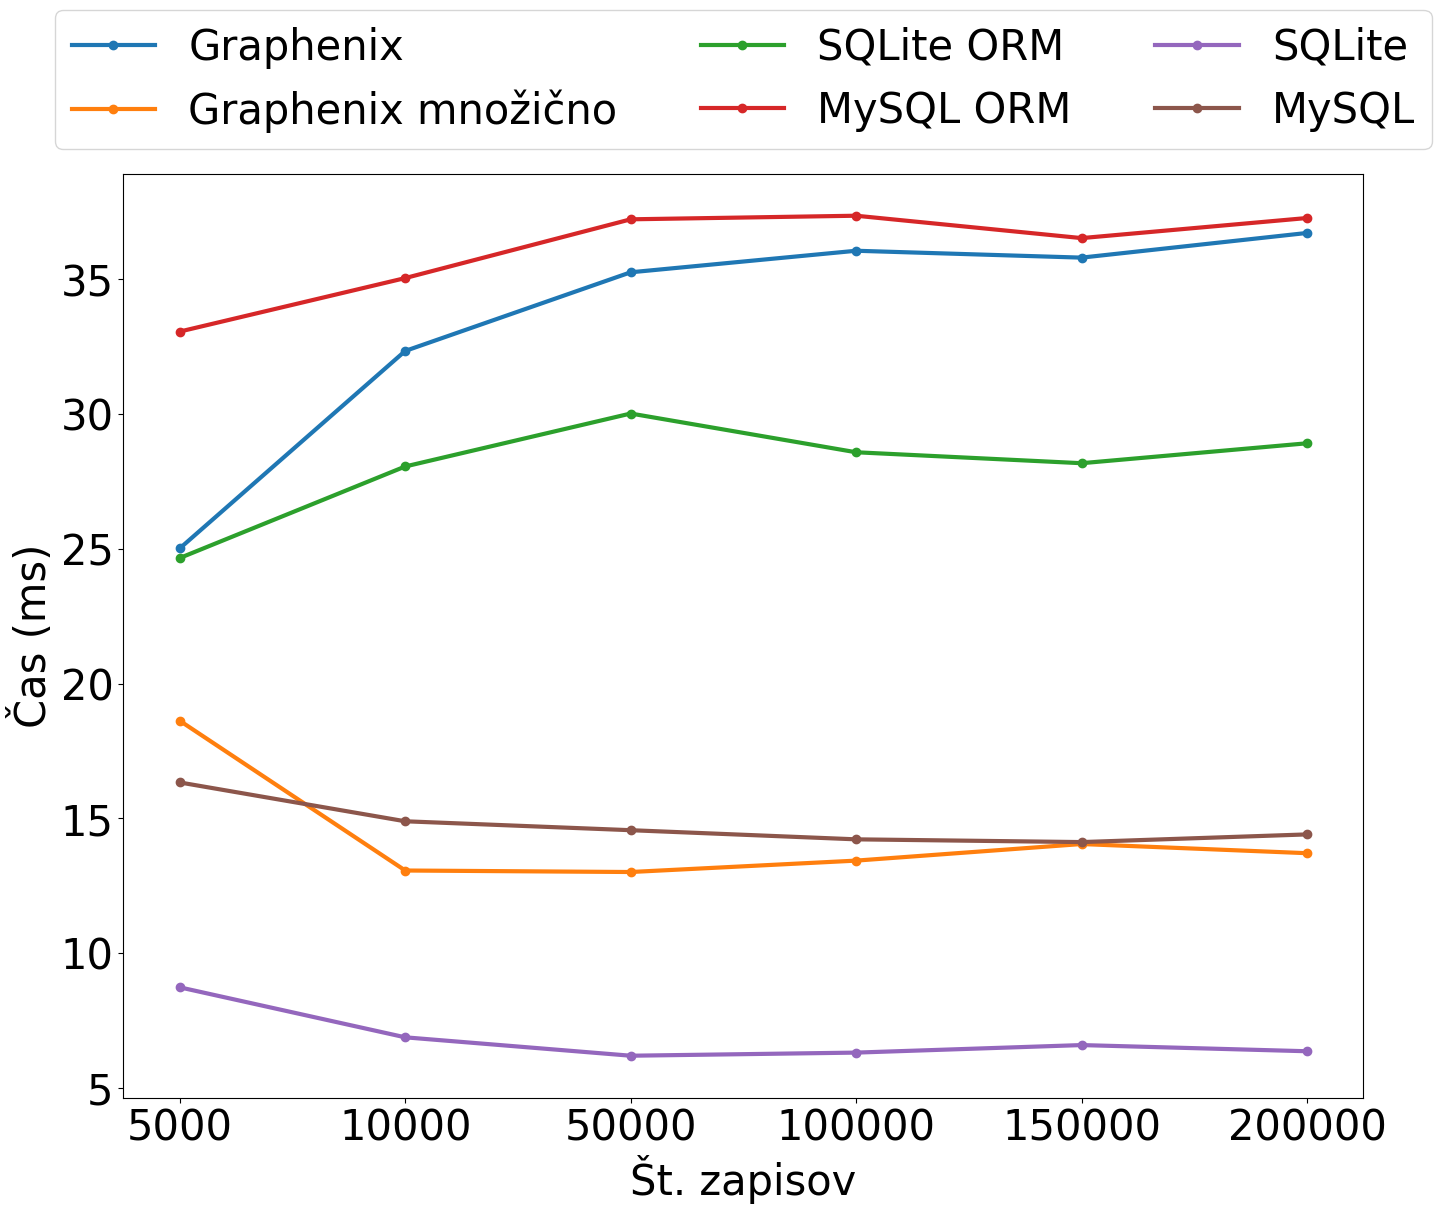
\includegraphics[height=4cm]{singleinsert.png}
            \vline
            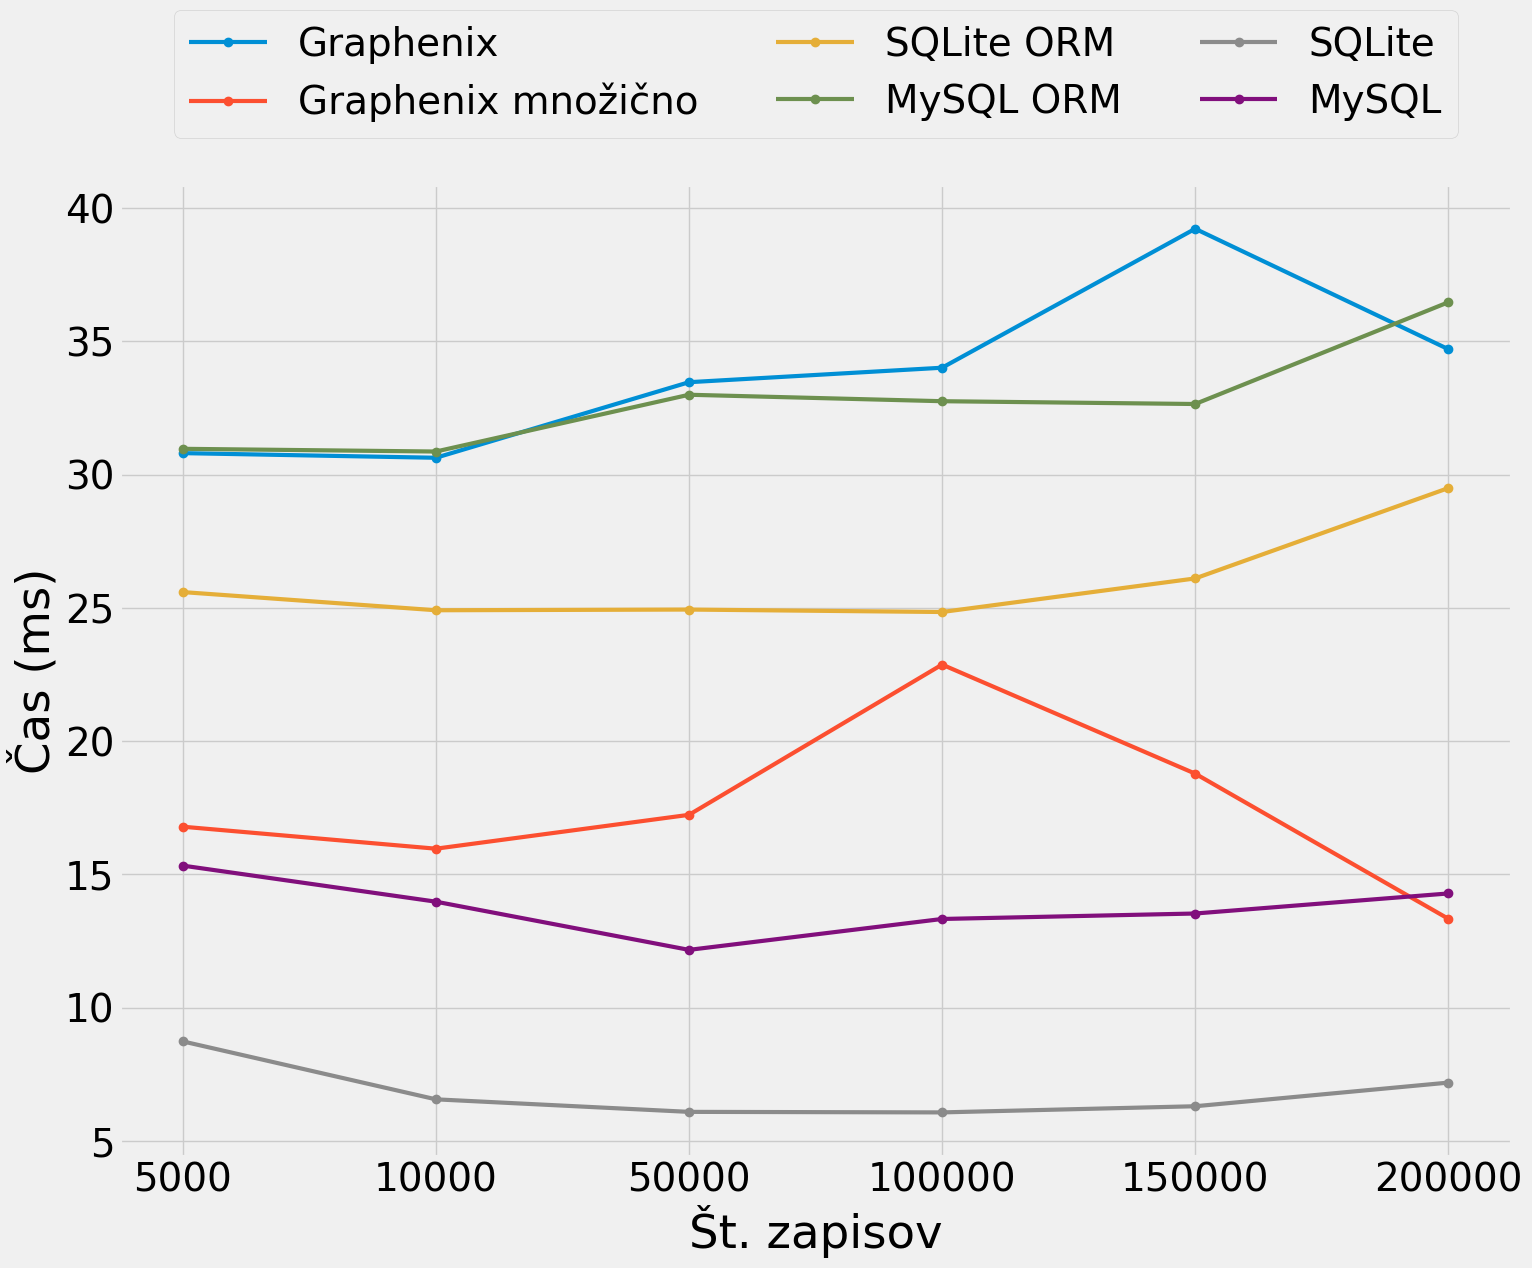
\includegraphics[height=4cm]{indexinsert.png}
    \end{frame}

    \subsection{Velikost podatkovne baze na disku}
    \begin{frame}
        \frametitle{Velikost podatkovne baze na disku}
            \centering
            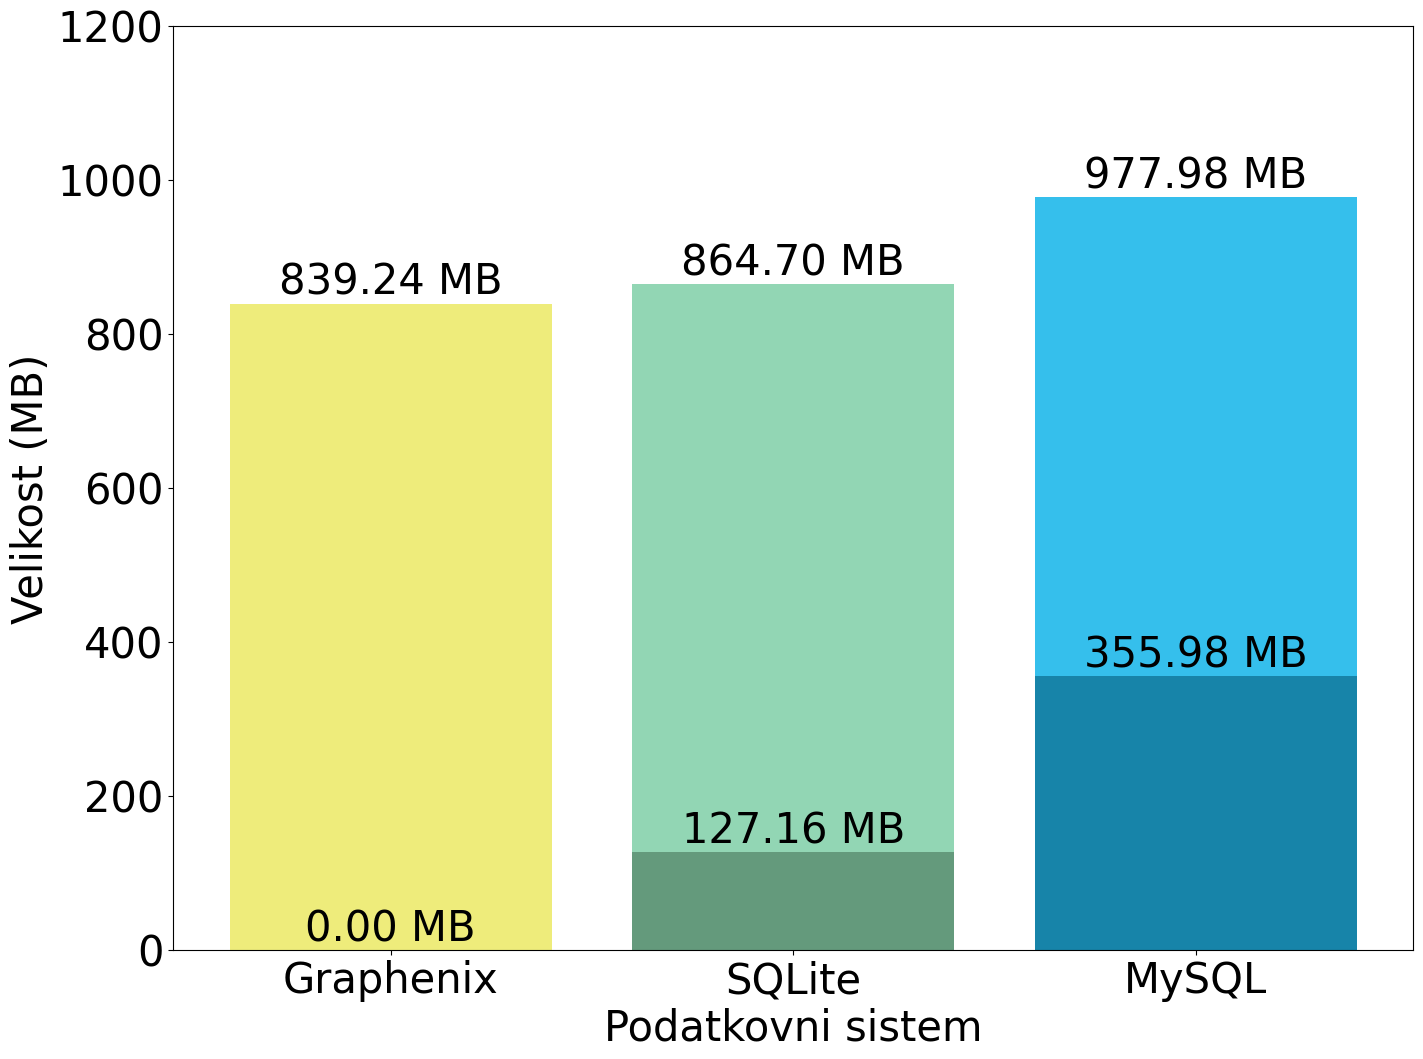
\includegraphics[height=6cm]{sizes.png}
    \end{frame}

    \subsection{Poizvedovanje}
    \begin{frame}
        \frametitle{Brez omejitev, s filtrom, s povezavami, agregacijsko}
        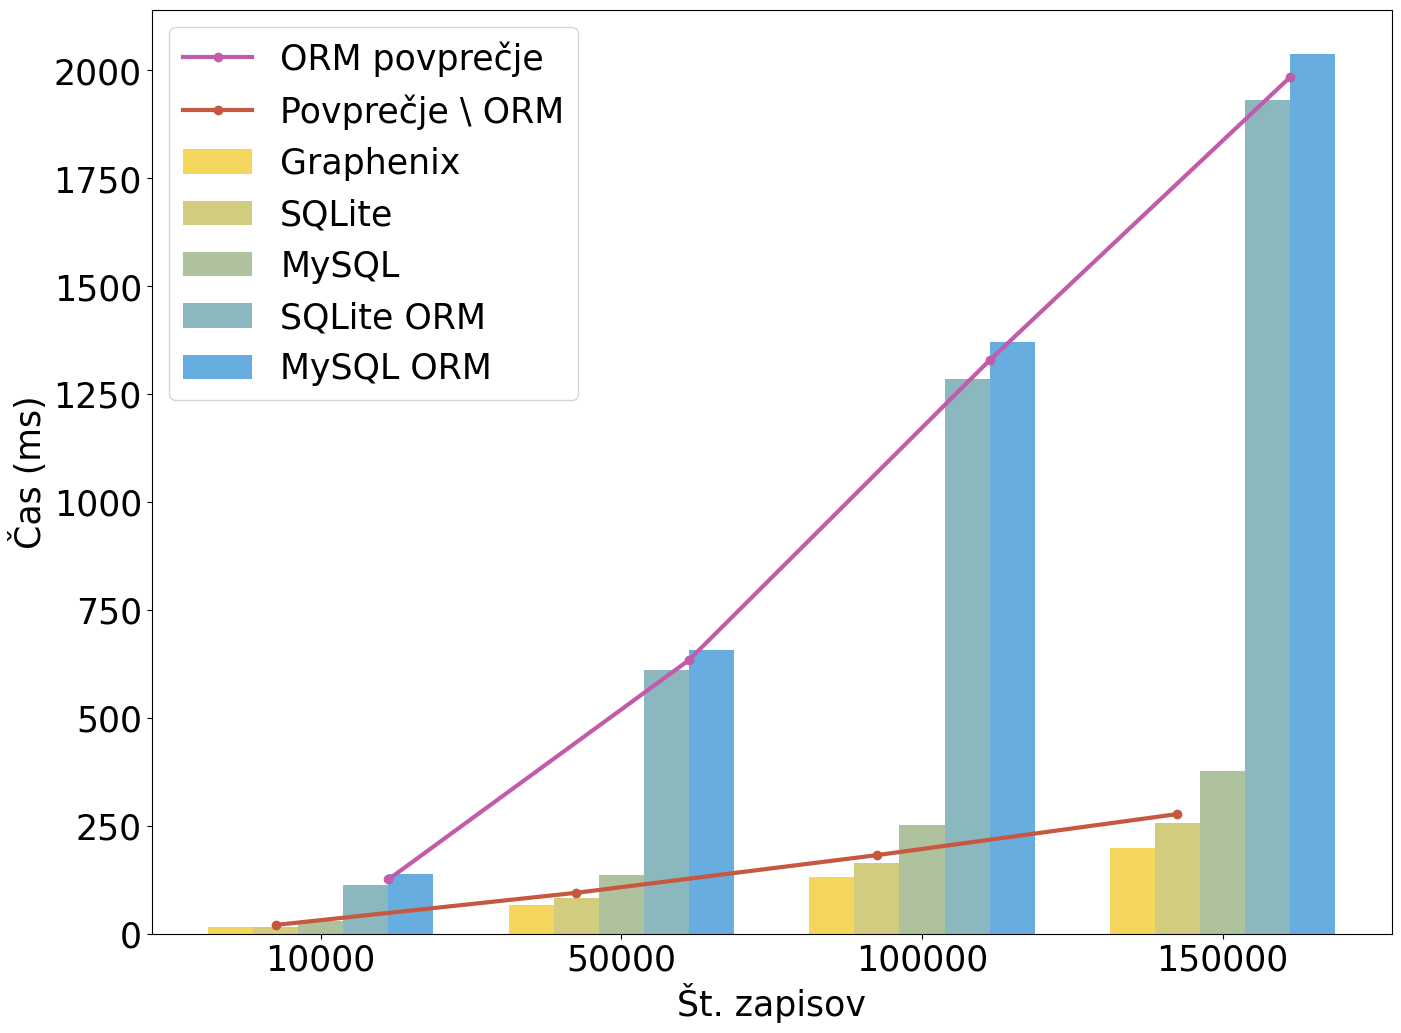
\includegraphics[height=3.2cm]{singleread.png}
        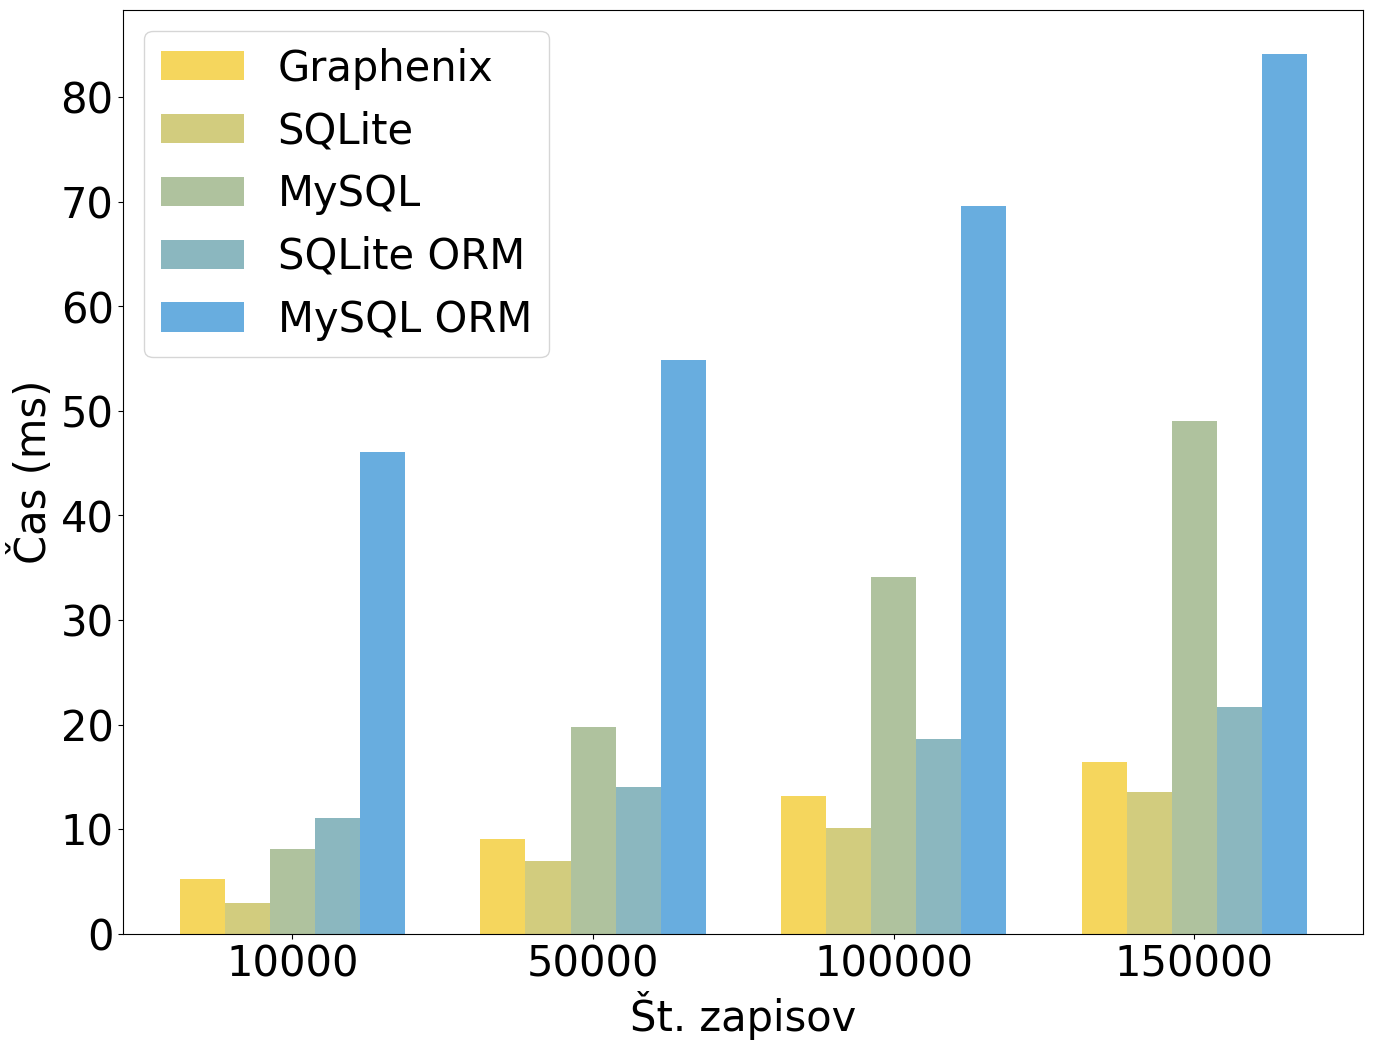
\includegraphics[height=3.2cm]{queryread.png}
        \hline
        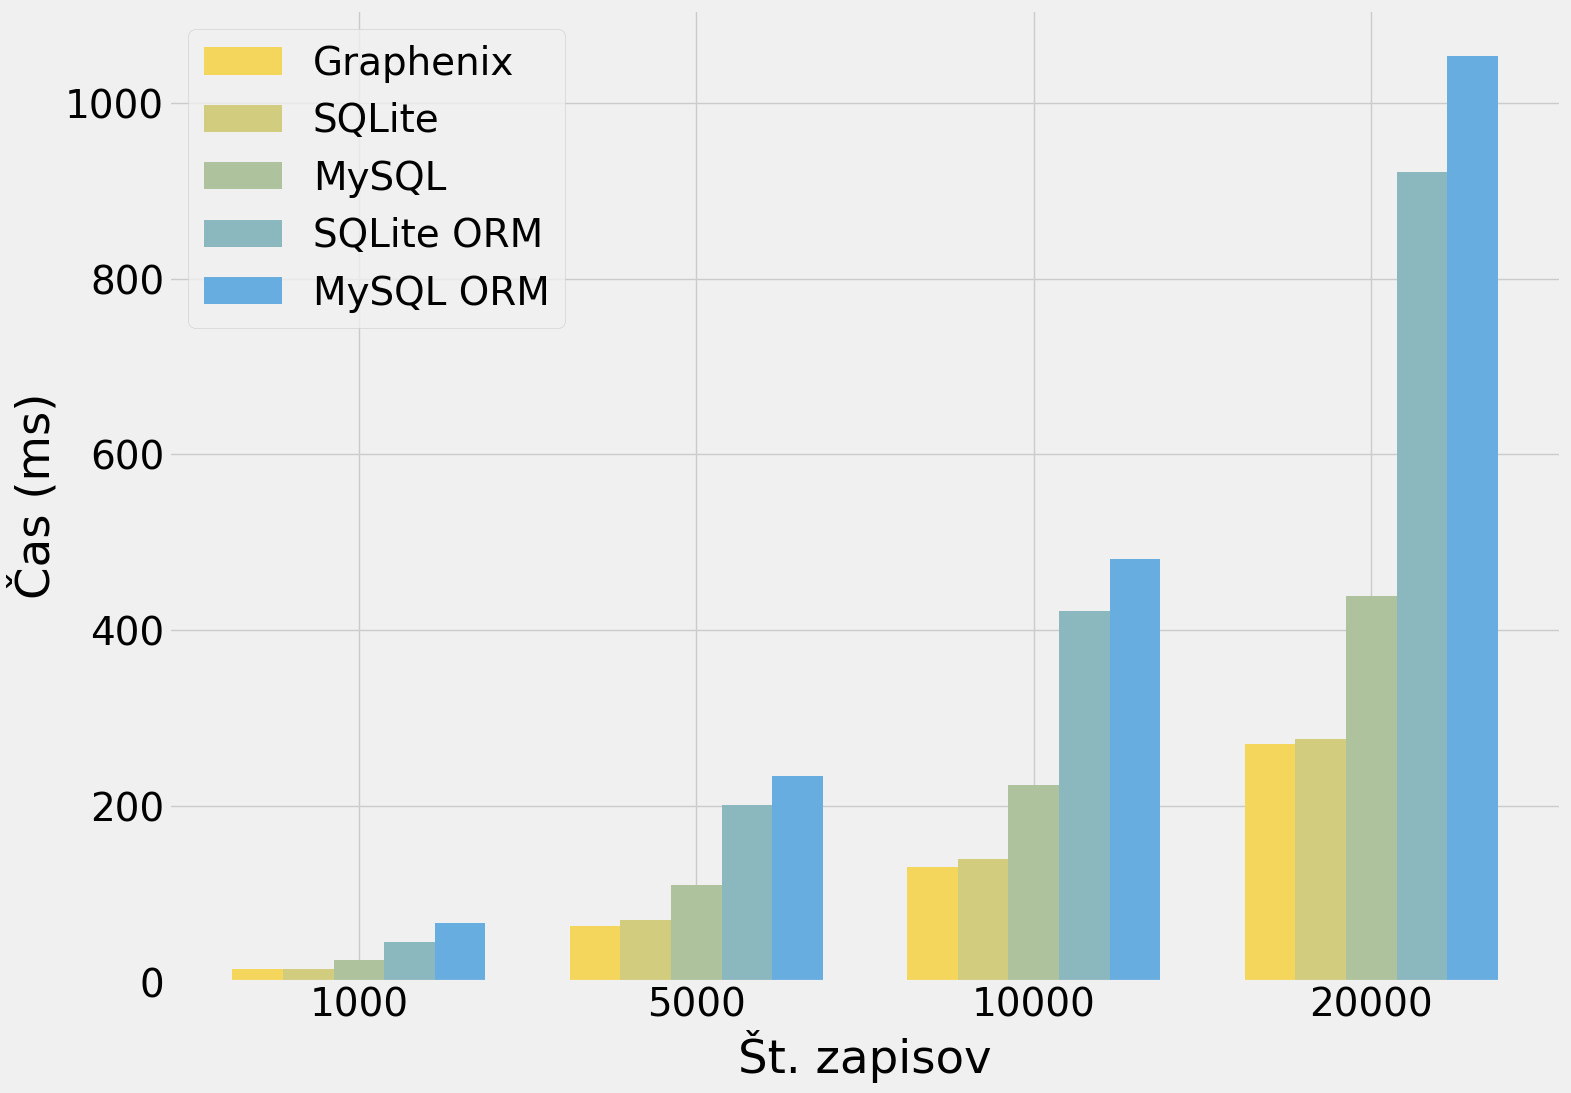
\includegraphics[height=3.2cm]{join.png}
        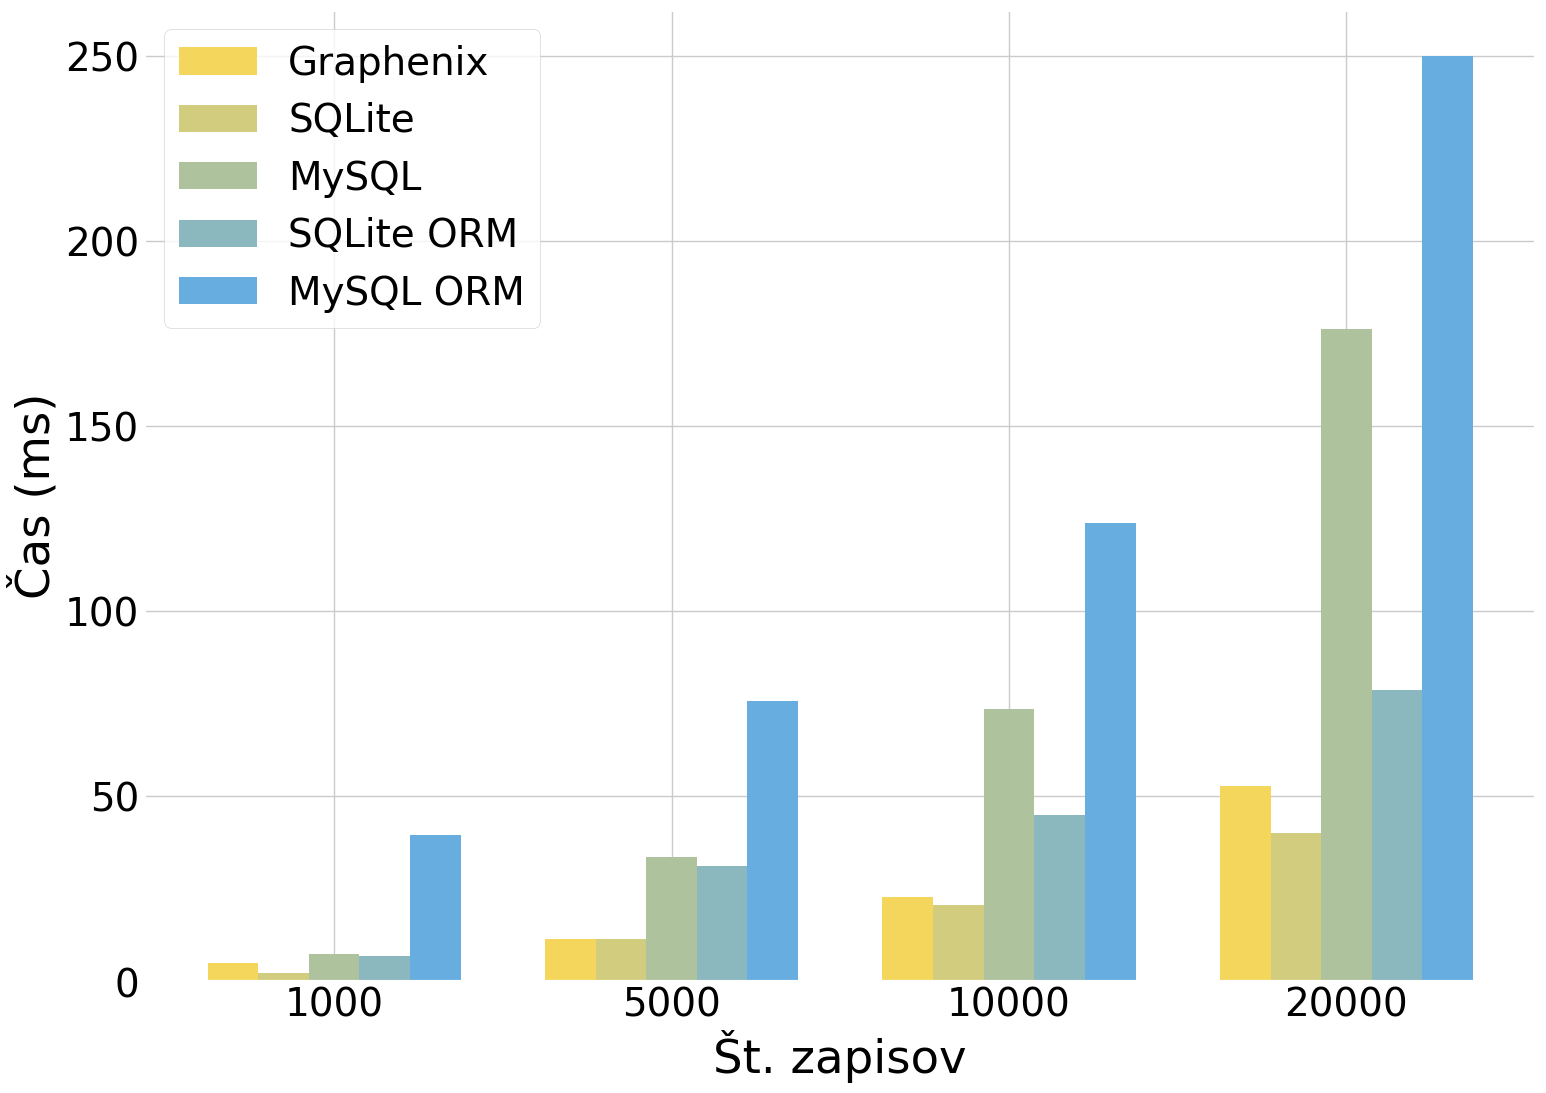
\includegraphics[height=3.2cm]{agg.png}
    \end{frame}

    \subsection{Uporaba indeksiranja}
    \begin{frame}
        \frametitle{Indeksiranje pred in po optimizaciji ($10^5$ zapisov)}
            \centering
            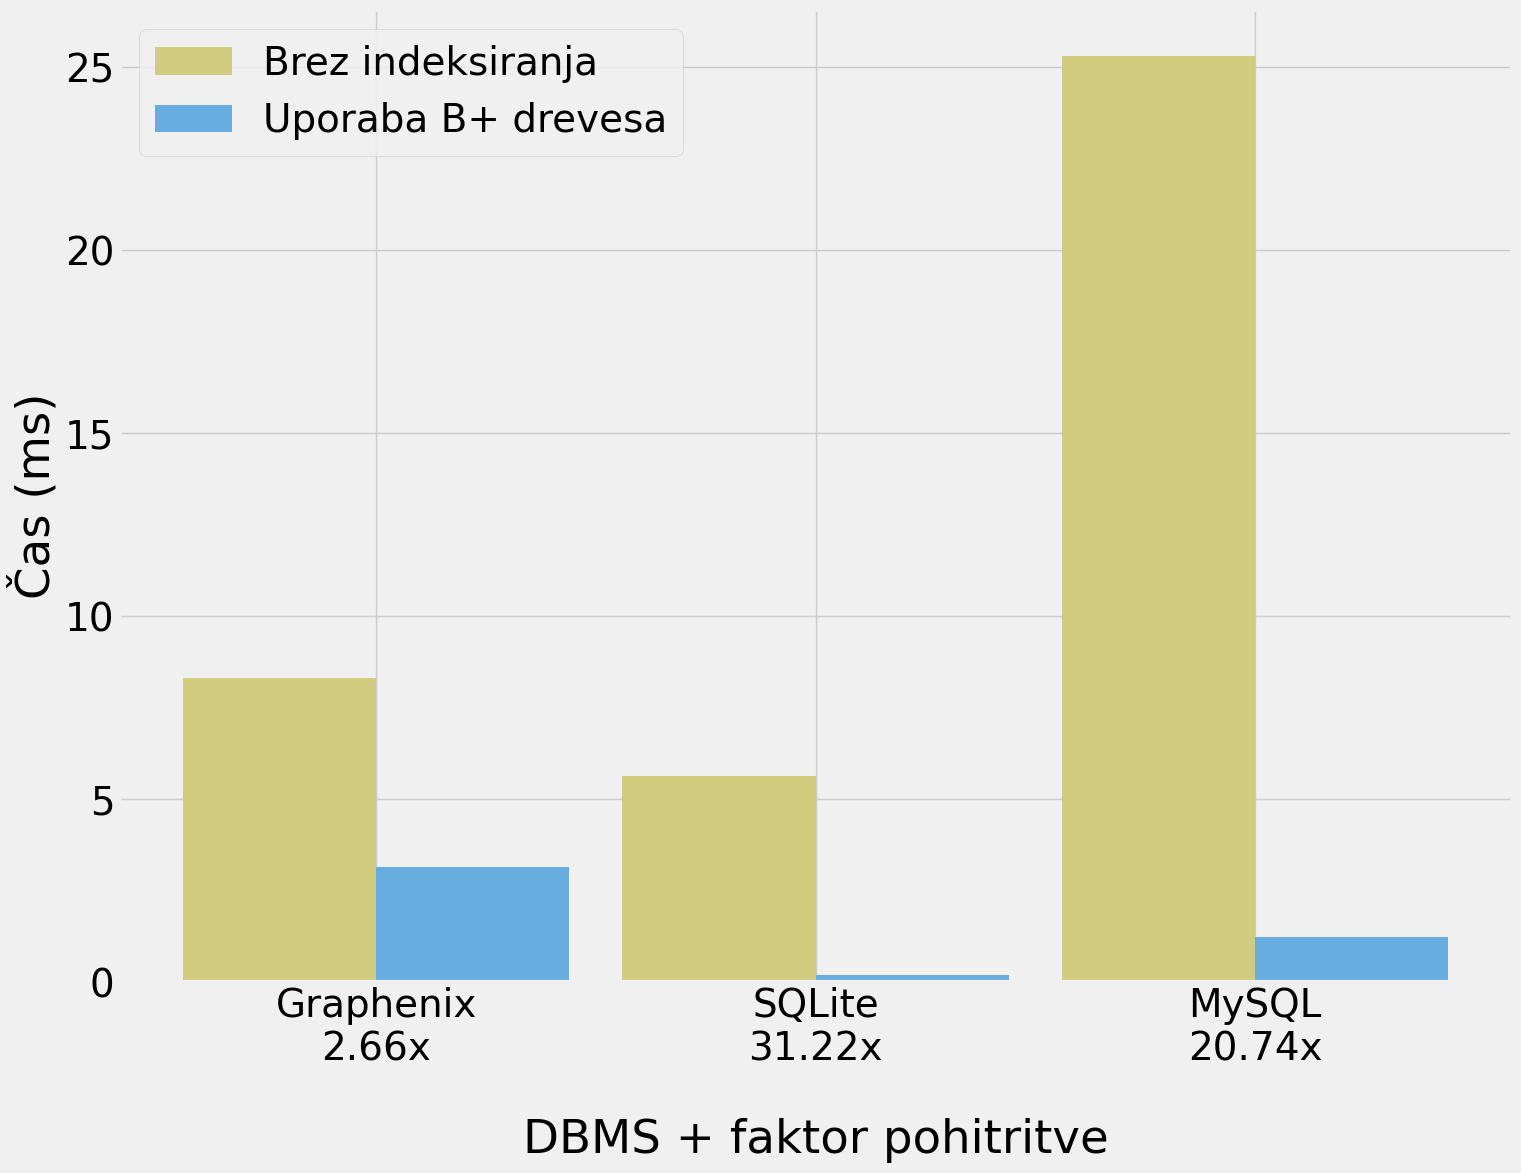
\includegraphics[height=4cm]{indexing_speedup_100000.png}
            \vline
            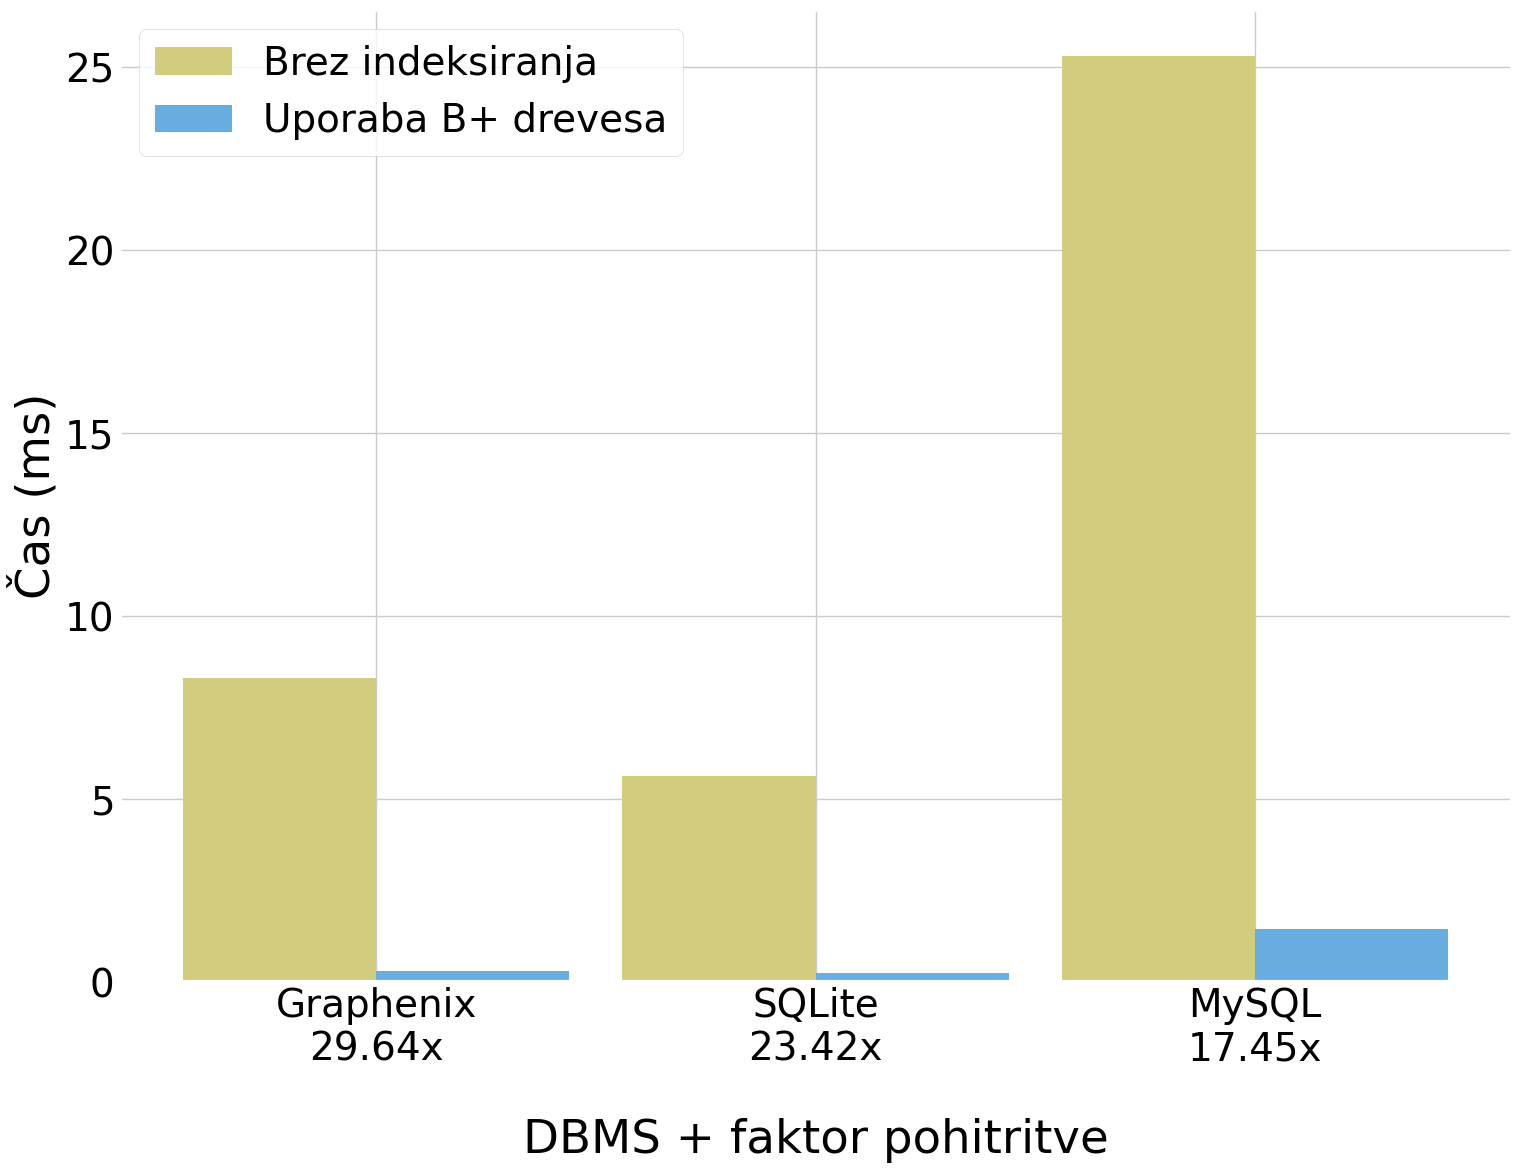
\includegraphics[height=4cm]{indexing_speedup_100000_v2.png}
    \end{frame}

    \begin{frame}
        \frametitle{Indeksiranje nad večjo bazo podatkov ($10^6$ zapisov)}
            \centering
            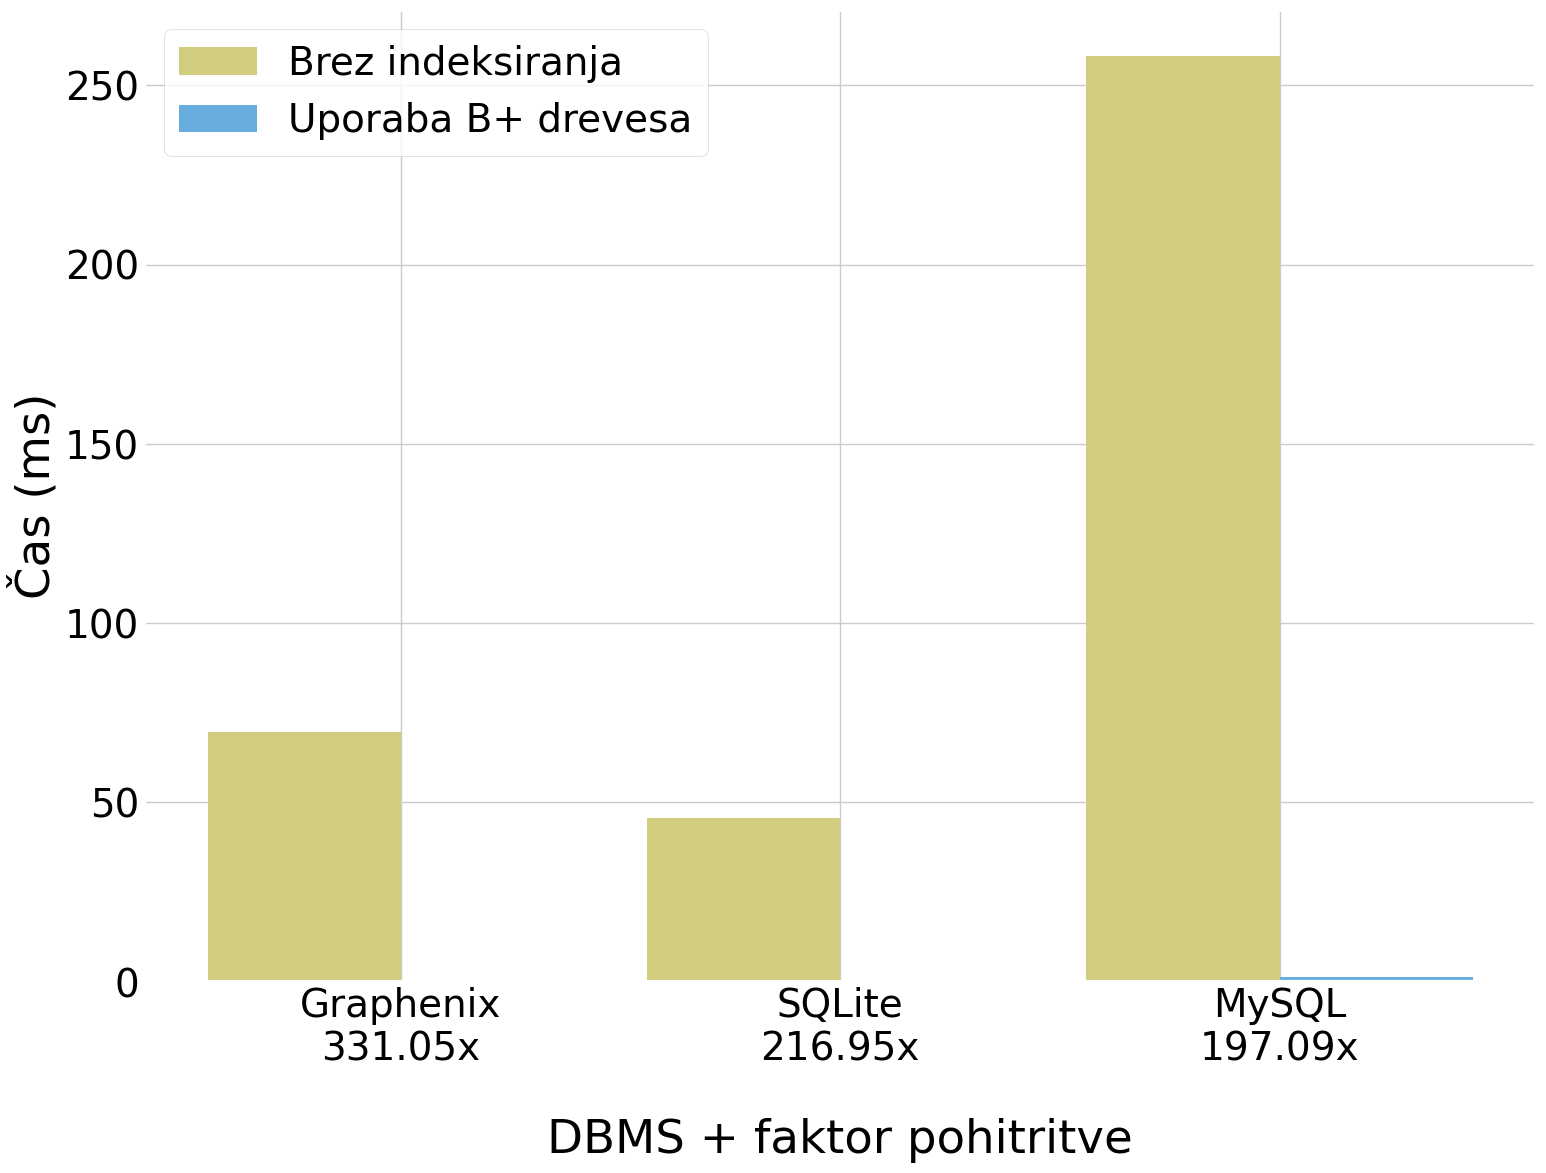
\includegraphics[height=6cm]{indexing_speedup_1000000_v2.png}
    \end{frame}

\section{Sklepne ugotovitve}
\begin{frame}
\frametitle{Sklepne ugotovitve}
    \begin{itemize}
        \item Kje je rešitev uporabna?
        \item Kaj rešitvi manjka za uporabo v produkcijskem okolju?
        \item Ali je bil razvoj uspešen?
    \end{itemize}
\end{frame}


\begin{frame}
\Huge{\centerline{Hvala za pozornost}}
\end{frame}

%----------------------------------------------------------------------------------------

\end{document} 